\begin{Aufgabe}[8]
Hinweis: Alle Teilaufgaben können unabhängig voneinander bearbeitet werden.

\begin{enumerate}
	\item
		Geben Sie eine lineare Differenzialgleichung an, die die Fundamentallösung
		\[
			y(x) = \e^{-2 \, x}
		\]
		besitzt.
		
		\Loesung{80mm}{
		Eigenwert $\lambda_1 = -2$:\hfill\Punkte{2 P}
		\[
			y'(x) = -2 \ y(x) 
		\]
		}
	\item
		Bei welchen Störfunktionen $r$ tritt bei der Differenzialgleichung
		\[
			y'' + 9 \, y = r(x)
		\]
		Resonanz auf?
		Bitte kreuzen Sie den entsprechenden Eintrag an:
		
		\ifLoesung 
		\begin{tabular}{p{0.3\textwidth}p{0.2\textwidth}p{0.2\textwidth}}
			$r(x) = \e^{-9 \, x}$ & $\square$             Resonanz & {\textcolor{red}X} keine Resonanz\\
			$r(x) = \e^{  9 \, x}$ & $\square$             Resonanz & {\textcolor{red}X} keine Resonanz\\
			$r(x) = 3 \, \cos(x)$ & $\square$             Resonanz & {\textcolor{red}X} keine Resonanz\\
			$r(x) = \cos(3 \, x)$ & {\textcolor{red}X} Resonanz &            $\square$  keine Resonanz\\
		\end{tabular}
		\hfill\Punkte{2 P}
		\else
		\begin{tabular}{p{0.3\textwidth}p{0.2\textwidth}p{0.2\textwidth}}
			$r(x) = \e^{-9 \, x}$ & $\square$ Resonanz & $\square$ keine Resonanz\\
			$r(x) = \e^{  9 \, x}$ & $\square$ Resonanz & $\square$ keine Resonanz\\
			$r(x) = 3 \, \cos(x)$ & $\square$ Resonanz & $\square$ keine Resonanz\\
			$r(x) = \cos(3 \, x)$ & $\square$ Resonanz & $\square$ keine Resonanz\\
		\end{tabular}
		\fi
		
		\newpage
		
		\item
			Die folgenden beiden Abbildungen zeigen den zeitlichen Verlauf der Zustände $z_1(t)$ und $z_2(t)$:
			
			\newcommand{\zeins}[1]{1+exp(-0.5*#1)*cos(deg(3*#1))}
			\newcommand{\zzwei}[1]{-0.5*exp(-0.5*x)*cos(deg(3*x))-3*exp(-0.5*x)*sin(deg(3*x))}
			
			\par
			
			\quad 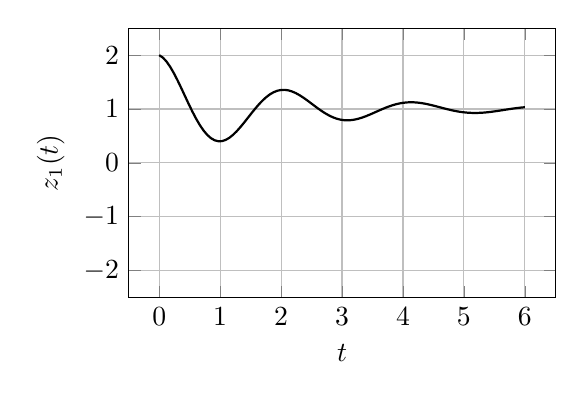
\begin{tikzpicture}
	\begin{axis}[
		xlabel={$t$},
		ylabel={$z_1(t)$},
		xmin=-0.5, xmax=6.5,
		ymin=-2.5, ymax=2.5,
		domain=0:6,
		samples=100,
		grid=major,
		width=7cm,
		height=5cm,
		xtick={0, 1, 2, 3, 4, 5, 6},
		ytick={-2, -1, 0, 1, 2}
		]
		\addplot [
		black,
		thick
		] {\zeins{x}};
	\end{axis}
\end{tikzpicture} \quad \quad \quad 		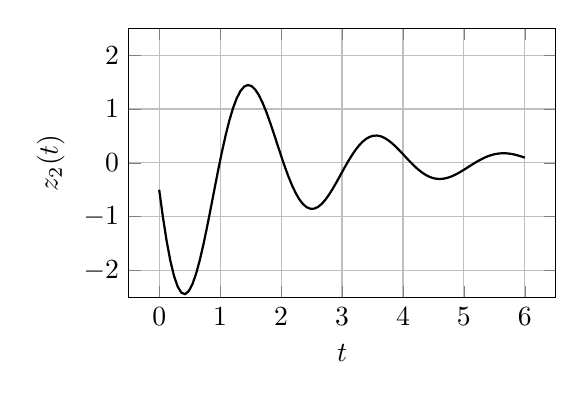
\begin{tikzpicture}
	\begin{axis}[
		xlabel={$t$},
		ylabel={$z_2(t)$},
		xmin=-0.5, xmax=6.5,
		ymin=-2.5, ymax=2.5,
		domain=0:6,
		samples=100,
		grid=major,
		width=7cm,
		height=5cm,
		xtick={0, 1, 2, 3, 4, 5, 6},
		ytick={-2, -1, 0, 1, 2}
		]
		\addplot [
		black,
		thick
		] {\zzwei{x}};
	\end{axis}
\end{tikzpicture}
			
			\par
			
			Welche der folgenden vier Abbildungen zeigt den richtigen Verlauf des Phasenporträts?
			Bitte begründen Sie Ihre Antwort!

			\par

			\quad \input{../M2_IT/m2_it_ss_24_kurzaufgaben_fig3.tex} \hspace*{40mm} 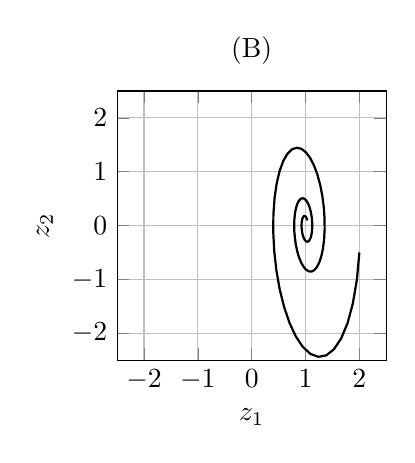
\begin{tikzpicture}
	\begin{axis}[
		title={(B)},
		xlabel={$z_1$},
		ylabel={$z_2$},
		xmin=-2.5, xmax=2.5,
		ymin=-2.5, ymax=2.5,
		domain=0:6,
		samples=100,
		grid=major,
		width=5cm,
		height=5cm,
		xtick={-2, -1, 0, 1, 2},
		ytick={-2, -1, 0, 1, 2}
		]
		\addplot [
		black,
		thick
		] (
		{\zeins{x}}, 
		{\zzwei{x}}
		);
	\end{axis}
\end{tikzpicture}
			
			\par

			\quad 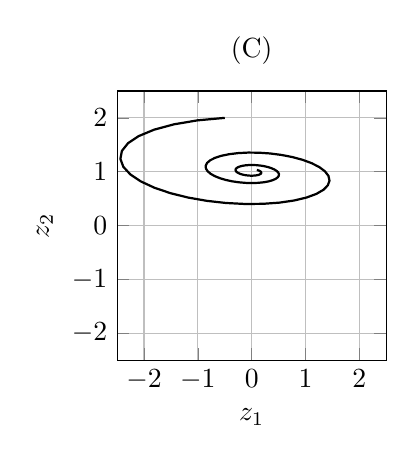
\begin{tikzpicture}
	\begin{axis}[
		title={(C)},
		xlabel={$z_1$},
		ylabel={$z_2$},
		xmin=-2.5, xmax=2.5,
		ymin=-2.5, ymax=2.5,
		grid=major,
		domain=0:6,
		samples=100,
		width=5cm,
		height=5cm,
		xtick={-2, -1, 0, 1, 2},
		ytick={-2, -1, 0, 1, 2}
		]
		\addplot [
		black,
		thick
		] (
		{\zzwei{x}},
		{\zeins{x}}
		);
	\end{axis}
\end{tikzpicture} \hspace*{40mm} \input{../M2_IT/m2_it_ss_24_kurzaufgaben_fig6.tex}

	\Loesung{}{
		Die Spirale endet in der Nähe des Punktes mit den Koordinaten $(1 \mid 0)$.
		Die Werte des Zustands $z_1$ bewegen sich zwischen $0$ und $2$.
		Somit zeigt Abbildung (B) den richtigen Verlauf.
		\hfill\Punkte{2 P}
	}
		
	\newpage
	
		\item
			Beurteilen Sie den folgenden Dialog mit ChatGPT 3.5.
			Sind die Berechnungen und die Behauptungen von ChatGPT korrekt?
			Es genügt den Fehler zu finden, die richtige Lösung muss nicht bestimmt werden!
		
			\textbf{You:} Wie lautet die Lösung des Anfangswertproblems (AWP)
			\[
				x' \cdot x = t, \quad x(0) = 1 \, ?
			\]
		
			\textbf{ChatGPT 3.5:} Um das AWP zu lösen, können wir das Verfahren der Trennung der Variablen verwenden.
		
			1. Trenne die Variablen:
			\[ \frac{{dx}}{{x}} = t \, dt \]
			2. Integriere beide Seiten:
			\[ \int \frac{{dx}}{{x}} = \int t \, dt \quad \Longleftrightarrow \quad \ln|x| = \frac{{t^2}}{2} + C \]
			3. Löse nach \(x\) auf:
			\[ |x| = e^{\frac{{t^2}}{2} + C} \]
			Da \(x(0) = 1\), setzen wir \(t = 0\) und lösen für \(C\):
			\[ |1| = e^C \quad \Longleftrightarrow \quad C = 0 \]
			4. Setze \(C\) ein und berücksichtige das Betragszeichen:
			\[ |x| = e^{\frac{{t^2}}{2}} \quad \Longleftrightarrow \quad  x = \pm e^{\frac{{t^2}}{2}} \]
			Da \(x(0) = 1\), wählen wir das positive Vorzeichen:
			\[ x(t) = e^{\frac{{t^2}}{2}} \]
			
		\Loesung{}{
			Die Trennung der Variablen ist falsch, richtig ist:
			\hfill{\Punkte{2 P}}
			\[ x \cdot \frac{dx}{dt} = t \quad \Longleftrightarrow \quad \int x \, dx = \int t \, dt \]
			Hinweis: ChatGPT 4.0 bestimmt die Lösung des AWP korrekt!
		}
\end{enumerate}
\end{Aufgabe}

\newpage

\endinput